%---------------------------------------------------------------------------------------------------
%		main.tex
%
%	This is the main file of the chapter that talk about a possible software architecture.
%
%	Author: Andrea Meneghinello
% Version: 0.1
%	Table of changes:
%		21/03/2016 -> document definition
%---------------------------------------------------------------------------------------------------
\chapter{Multi-tenant \& elastic architecture}
\label{cap:architecture}
After having analysed, in Chapter \ref{cap:measurements}, two virtualization alternative techniques that
a \ac{paas} provider can make available to us, we want to conclude our discussion talking about the other
side of the coin to obtain elasticity: the software architecture.

As we said in Chapter \ref{cap:elasticity}, elasticity can be obtained by blending together a virtualization
layer (that exploits as better as it can the underlying hardware) and a good software architecture (that is
able to take advantage of the functionalities provided by the virtualization layer).

Thus, in this chapter we want to discuss about \acf{soa} as a possible solution for building elastic and
multi-tenant applications or services. In particular in Section \ref{sec:architecture-introduction} we will
do a brief introduction about the state-of-the-art in software architectures to understand why they are not
good candidates to obtain elasticity. Hereafter, in Section \ref{sec:architecture-soa} we will introduce
the concept of \ac{soa} and we will explain how we can reconsider it in the cloud landscape. Finally, in
Section \ref{sec:architecture-proposal} we will discuss about a possible software architecture that can lead 
us to build elastic and multi-tenant applications combined with Docker containers.

%---------------------------------------------------------------------------------------------------
%		introduction.tex
%
%	This is the main file of the chapter that talk about elasticity.
%
%	Author: Andrea Meneghinello
% Version: 0.1
%	Table of changes:
%		17/03/2016 -> document definition
%---------------------------------------------------------------------------------------------------
\section{Introduction}
\label{sec:elasticity-introduction}
A requirement for distributed services is availability: they must remain regularly available to be
used by as many customers as needed with \keyword{acceptable performance} and \keyword{scalability}.
Distributed services and systems have always been required to be scalable. Replication of services
components, in order to balance the workload arriving to each replica, has been the chosen approach.

Services needed to be carefully designed in order to minimize synchronization needs among their
components with the aim of not blocking their execution. Evidently, unlimited scalability could not be
achieved since it requires infinite infrastructure resources. So, traditionally, scalability of a
service depends on its software architecture being limited by the amount of hardware resources secured
in the data-centre where it was deployed.

As we have seen in the previous chapter, the advent of cloud computing partially broke those limits, but
elasticity management remains not trivial.

According to the \ac{nist} definition (given in Section
\ref{sec:background-cloudComputing-cloudServiceModels}), \ac{paas} gives freedom to the customer regarding
application reconfiguration, since end-users should only deal with the general ``configuration settings
for the application-hosting environment'' but do not need to worry about the mechanism being needed
for implementing those reconfigurations. Reconfiguration management is the responsibility of \ac{paas}
providers. Since every cloud service should be elastic (accordingly with cloud definition), this mean
that \ac{paas} providers should deal with many mechanism that automate the service scalability and
adaptability.

However, the level of automation needed to approach a cost-optimal exploitation of the service is still
changing nowadays because of the many aspects that should be considered. On one hand, scalability
decisions must match what has been stated in the \ac{sla}. This means that those decisions should be
taken as soon as the workload or the service performance starts to vary, which strongly suggests the
need to include some workload prediction mechanism. Nevertheless, forecasting techniques are not perfect
hence, they should be complemented with other reactive mechanism; e.g. when the resulting service
performance level do not comply with what is being specified in the \ac{sla} or lead unnecessary
over-provisioning costs, service providers should take appropriate actions. Those actions may consist
in adding service instances or migrating those instances to better \ac{vm}s when service capacity
should be increased, or in the opposite case, in releasing instances when service capacity need to be
decreased.

One of the regular dimensions in \ac{sla}s is availability. Successful distributed services are
concurrently used by many customers. Service providers should guarantee service continuity, otherwise
service clients will not rely on that provider and they will look for another, more reliable, one.
Unfortunately, since complex software systems are always in need of modification, both platform and
service components need to be eventually updated in order to fix bugs, remove security vulnerabilities
or enhance their functionality. This software upgrading process might put at risk the availability levels
specified in a \ac{sla}. So, this is another source of trouble for service providers.



%---------------------------------------------------------------------------------------------------
%		introduction.tex
%
%	This is file contains an introduction about the SOA architectural desing.
%
%	Author: Andrea Meneghinello
% Version: 0.1
%	Table of changes:
%		21/03/2016 -> document definition
%---------------------------------------------------------------------------------------------------
\section{\acs{soa} re-visitation}
\label{sec:architecture-soaRevisitation}
In the following Sections we want to review the \ac{soa} architecture in order to exploit its main
characteristics. We will use the re-visitation later in our architecture in order to provide an
elastic and multi-tenant architecture deployable in the \ac{paas}.

\subsection{\acf{soa}}
A \acf{soa} is an architectural model for the creation of systems that reside over a network and
focus their attention over the concept of \keyword{services}. A system built following the \ac{soa}
philosophy is made of applications called services. They are well defined, independent from each
other and they can reside on multiple computers linked in a network.

Each service makes a certain functionality available, and can utilize the ones made available by other
services. Though this architecture, we are able to build more sophisticated applications starting from
elementary components. Its work model is illustrated in Figure \ref{img:architecture-soaRevisitation-workmodel}

\begin{figure}
	\centering{}
	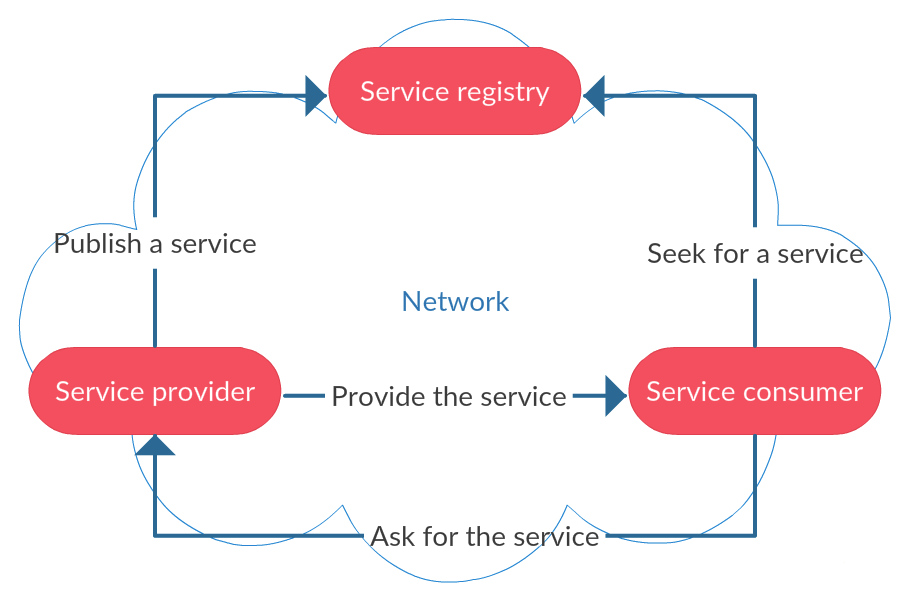
\includegraphics[width=0.7\textwidth]{chapters/architecture/images/soa-workmodel.png}
	\caption[Example of \acs{soa} architecture]{Example of \acf{soa} architecture.}
	\label{img:architecture-soaRevisitation-workmodel}
\end{figure} 

\ac{soa} abstraction is not related to any specific technology, but it simply defines some properties 
that are oriented to the \keyword{reuse} and to the \keyword{integration} in a heterogeneous environments
of its base components.

In particular, each service must have the following properties (illustrated in Figure 
\ref{img:architecture-soaRevisitation-characteristics}):

\begin{itemize}
	\item{\keyword{service discoverability}: a service must be retrieved basing on its interface and
		called at run-time;}
	\item{\keyword{service autonomy}: every service must be well defined, complete and independent
		from the context or from the status of other services;}
	\item{\keyword{standardized service contract} and \keyword{service abstraction}: services must
		be defined in terms of what they do, abstracting them from the technologies used to implement
		them. This determines the independence from both the used programming language and the \acs{os}
		on which they are running. It is not necessary to know how a service is implemented but only
		the offered functionalities.}
	\item{\keyword{service loose coupling}: an architecture is loosely coupled if the dependencies
		between its components are limited. Thus, we have to made services that depends least as possible
		by other making the system flexible and easily customizable;}
	\item{\keyword{service reusability}: each service must be made available on the network through
		the publication of its interface and made accessible in a transparent way (location awareness);}
	\item{\keyword{service statelessness}: services minimize the resource consumption and delegate
		the status information management when necessary;}
	\item{\keyword{service composability}: in a \ac{soa} architecture the applications are the result of
		the composition of many services. This is the reason that leads us to build independent services
		in order to obtain the maximum re-usability. The creation of applications or more complex
		services through composability is defined as \keyword{service orchestration}.}
\end{itemize}

\begin{figure}
	\centering{}
	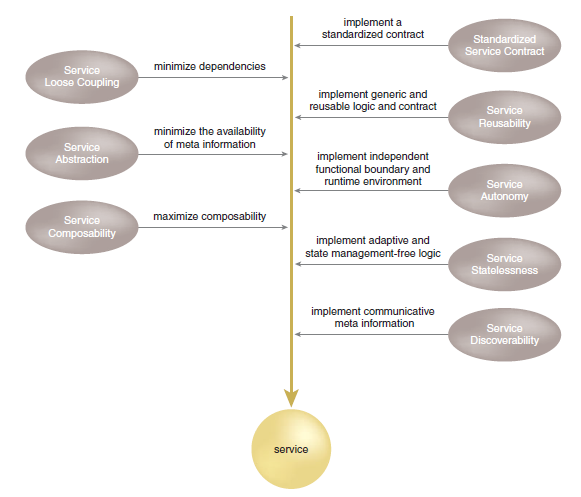
\includegraphics[width=0.8\textwidth]{chapters/architecture/images/soa-characteristics.png}
	\caption[Service oriented logic]{Service oriented logic \cite{serviceCharacteristics}.}
	\label{img:architecture-soaRevisitation-characteristics}
\end{figure}

\subsubsection{Difference with cloud computing model}
\label{sec:architecture-soaRevisitation-compatibility}
\ac{soa} architecture was born in the pre-cloud era, thus it is not conceived to address cloud computing
issues. But \ac{caa} and \ac{soa} share some characteristics that bring us to consider \ac{soa}'s base
philosophy while building our architecture.

First, both emphasize the \keyword{service concept}. By definition, a service is made up by smaller parts
that do the job to build the final output, everyone using the \keyword{delegation} system. With that methodology,
people can use the services without worrying about their implementation details and their scalability. In
addiction, services can be shared by multiple applications and users, thus optimizing resource consumption,
and enabling the concept of multi-tenancy (see Section \ref{sec:elasticity-multiTenancy})

Second, both promote the ``\keyword{loose coupling}'' principle. Each architecture demands minimum
dependencies among different parts of the system. As a result, any single change on one part of the system
has limited impact on the overall system.

Since \ac{soa} was born in the pre-cloud era it presents some differences that bring us to reconsider its
base philosophy before starting its adoption inside the cloud model. Both differ in term of the concepts
of \keyword{service} and \keyword{infrastructure}.

The services in \ac{soa} mainly focus on business. Each service may represent one aspect of the business and
combined together, these services consist of a business application or solution. In this sense, the
\keyword{services are horizontal}. Basically \ac{soa} was regarded as a single, monolithic entity,
while in cloud we have to see it as an elastic group of  multiple service instances. Actually, the services
in \ac{caa} must be mainly layered according to typical software stacks. The lower services support the upper
services to deliver applications. Therefore, we call them \keyword{vertical services}.

\ac{soa} is for application architectures. The dividing of different components is based on their roles in
the \ac{soa} applications. More often than not, we start with a business problem and then abstract out the
services. These services can be re-used by other applications in the future. Instead cloud computing is for
\acs{it} delivery, so the dividing of different services is based on their roles in a software stack that is
mostly well defined. We do not need a problem before defining the cloud services. Services can be easily
re-used by every applications.

In conclusion, \ac{soa} and cloud computing share many common principles, but also differ significantly
in their role in \acs{it} architecture. \ac{soa} is mainly an application architecture with horizontal
services; while cloud computing is an \acs{it} architecture with vertical services. The service orientation
paradigm supplies the \ac{saas} providers with the necessary support for the implementation of interoperable 
services but they can not be scaled as fast as needed because of their monolithic nature. Our proposal is
to cover this lack with the adoption of the subset of \ac{soa} called micro-service pattern.

\subsection{Micro-services}
\label{sec:architecture-soaRevisitation-microService}
As we argued in the previous section a classic \ac{soa} approach does not fit well with a cloud
architecture, but the base concept remains valid. Thus we have to revisit the definition of
service in order to make it fit with the cloud needs and possibly exploit as better as it can the
concept of elasticity provided by the model.

The main problem with services defined by the \ac{soa} approach is their size. More often than not
they are to coarse-grained to scale efficiently. Thus, a need for smaller service is risen: their
name is \keyword{micro-services}.

In computing, ``micro-services'' is a software architecture style in which complex applications are
composed of small, independent processes communicating with each other using language-agnostic 
\acs{api}s. These services are \keyword{small building blocks}, \keyword{highly decoupled} and 
\keyword{focused} on doing a small task, facilitating a modular approach to system-building.

Microservices are becoming the cloud architecture of choice because they offer the ability to 
loosely couple applications into discrete services that can be surgically changed without requiring
disruptive overhauls. This approach enables the responsiveness and rapid change needed by the business.
Thus, with them we are able to switch from horizontal services to vertical ones.

Given the results described given in Chapter \ref{cap:measurements}, we have chosen to base our
architecture on Docker containers and use the micro-services as a possible base solution to provide an
elastic and multi-tenant application deployed in the cloud.

\subsubsection{Main properties}
\label{sec:architecture-soaRevisitation-microServices-properties}
The main properties of a micro-services architecture are:

\begin{itemize}
	\item{services are easy to replace;}
	\item{services are organized around capabilities (e.g., user interface, recommendation,
		logistics, billing, etc.);}
	\item{services can be implemented using different programming languages, databases, hardware and
			software environments, depending on what fits best;}
	\item{architectures are symmetrical rather than hierarchical (producer - consumer).}
\end{itemize}
			
The philosophy of micro-services architecture essentially equals the Unix philosophy of ``Do one thing and do
it well''. Fundamentally:
			
\begin{itemize}
	\item{the services are small, fine-grained in order to perform a single function;}
	\item{the organization culture should embrace automation of deployment and testing. This eases the burden
		on management and operations;}
	\item{the culture and design principles should embrace failure and faults, similar to anti-fragile systems;}
	\item{each service is elastic, resilient, composable, minimal, and complete.}
\end{itemize}

\subsubsection{Requirements of a micro-services architecture}
\label{sec:architecture-soaRevisitation-microServices-requirements}
When we are going to design a micro-services architecture there are some aspects that we must respect in order
to build an application that meet the elasticity requirements illustrated in Section \ref{sec:elasticity-requirements}.
\citeauthor{microservicesCommandments} in \cite{microservicesCommandments} group all those concepts in the
so-called ``ten commandments'' of a micro-services architecture. They are:

\begin{enumerate}
	\item{\keyword{clean separation of stateless and stateful services}: having a clear separation from
		stateless and stateful services allow the developers to easily share the micro-services between
		different tenants; later in Section \ref{sec:architecture-propoasal-architecture-multiTenancy}
		we will discuss how it is possible to manage multi-tenancy in stateful services;}
	\item{\keyword{do not share libraries or \ac{sdk}}: heaving no shared libraries or \ac{sdk} between
		micro-services permit to developers to adopt the \ac{cicd} pipeline during development phases;}
	\item{\keyword{avoid host affinity}: no assumption have to be made on where our micro-services will
		be executed; this increase the portability of our micro-services;}
	\item{\keyword{focus on services with one task in mind}: building highly specialized micro-services
		increase their re-usability; furthermore scarcely the size of each micro-service will be big, so
		guarantee the elasticity becomes more easier;}
	\item{\keyword{use lightweight messaging protocol for communication}: micro-services have to be
		designed in order to be highly collaborative, so a critical aspect lies in the creation of
		communication protocols. These protocol must be as easy as possible and to avoid possible lock 
		and necessary synchronizations we must consider to use asynchronous channels communications
		like \ac{amqp}\footnote{\ac{amqp} is an open standard application layer protocol for
		message-oriented middleware} \cite{amqpProtocol};}
	\item{\keyword{design a well-defined entry point and exit point}: through the design of clear
		interfaces the micro-services are more easier to reuse by other services and does not require
		to understand their internal business logic; furthermore it makes it easy to debug and maintain
		the code;}
	\item{\keyword{implement a self-registration and discovery mechanism}: to rich high level of
		automation it is necessary to introduce the presence of a central authority (a registry) that
		contains all active services in order that other are able to find them; therefore it is necessary to
		introduce in the service life-cycle a mechanism that permit the subscribe and unsubscribe of
		the service from the registry;}
	\item{\keyword{explicitly check for rules and constraints}: in order to guarantee high \ac{qos}
		levels sometimes our services have to be supported by constraints (e.g. execute in systems with
		\ac{ssd});}
	\item{\keyword{prefer polyglot over single stack}: having micro-services highly specialized permit
		to developers to use the most appropriate set of technologies and environments to support them;
		the only two necessary thing to assure are: clear interfaces and good communication protocols;}
	\item{\keyword{maintain independent revision and build environments}: having separated micro-services
		permit to developers to easily maintain them correctly versioned and simplifies recover phases
		and the continuous development of each one.}
\end{enumerate}

%---------------------------------------------------------------------------------------------------
%		proposal.tex
%
%	This is file contains an introduction about the SOA architectural desing.
%
%	Author: Andrea Meneghinello
% Version: 0.1
%	Table of changes:
%		21/03/2016 -> document definition
%---------------------------------------------------------------------------------------------------
\section{Our proposal}
\label{sec:architecture-proposal}
With the revisited \ac{soa} approach described in Section \ref{sec:architecture-soaRevisitation}, now we
want to introduce a possible real architecture that is able to offer an elastic and multi-tenant service
to companies that operates in the textile and clothing business.

In Section \ref{sec:architecture-proposal-company} we will introduce the company which will build our
proposal at the end of this thesis, explaining a little bit its origin and its business vision. Later
in Section \ref{sec:architecture-proposal-architecture} we illustrate the designed architecture explaining
how it will be able to reach the elasticity requirements illustrated in Section \ref{sec:elasticity-requirements}.

\subsection{The scenario}
\label{sec:architecture-proposal-company}
Meneghinello \cite{meneghinelloHomePage} is a small business company which has focus its activities
on providing a service that permit to its final customers to customize suits, jackets, shirts at home.
The service has been designed to offer a convenience service for those professionals who assert haven't
time to spend searching clothes suitable with their work activities. 

\begin{figure}[h!]
	\centering{}
	
\includegraphics[width=0.3\textwidth]{chapters/architecture/images/meneghinello.png}
	\caption[Meneghinello's brand]{Brand of Meneghinello company \cite{meneghinelloHomePage}.}
	\label{img:architecture-proposal-scenario}
\end{figure}

The company was born with the idea that offering this kind of service at home was a great facilitator,
and for many years it has been a success factor. This was motivated because customers, like lawyers or
accountants and other have found this service very useful and fair with their return back (high-quality
products and high-level of service).

Given the presence of itinerant agents, who have to know a certain amount of data (physical measures,
previous purchases, proposal that they joined, biographical data, etc.) in order to satisfy the customer
needs, the request to access to that data everywhere and with any type of device is risen.

In addition, the company saw in the recent years the growth of different competitors, that started to offer
about the same service. Therefore it started to think to differentiate its business starting a production
a service that permit to the itinerant agents to have access to those data everywhere and with any type
of device.

The typical request made by those companies are the following:

\begin{itemize}
	\item{manage biographical data of their customers;}
	\item{manage purchase data;}
	\item{be visible on the web (having a web-site that describe the company);}
	\item{possibility to sell their product through a web-site;}
	\item{possibility to contact, by mail, their customers;}
	\item{manage the inbound mail.}
\end{itemize}

The author thought to exploit the opportunity of the thesis period to learn a technologies and architectural
patterns that are able to facilitate the construction and the maintenance of an elastic and multi-tenant
service. In the following section we will briefly introduce the designed architecture and we will explain
its major components and how, through these it is able to reach the elasticity requirement illustrated in
Section \ref{sec:elasticity-requirements}.

\subsection{Proposed architecture}
\label{sec:architecture-propoasal-architecture}
After reading the comparison evaluations illustrated in Chapter \ref{cap:measurements} and the concepts
discussed in Section \ref{sec:architecture-soaRevisitation} and we are now able to understand the proposed
architecture based on Docker containers. Figure \ref{img:architecture-proposal-architecture} illustrate an
overview of the proposal, that we are able to define as:

\begin{center}
	\begin{quote}
		``a collection of independent, autonomous containers participating in an application that defines
		the micro-services architecture.''
	\end{quote}
\end{center}

\begin{figure}
	\centering{}
	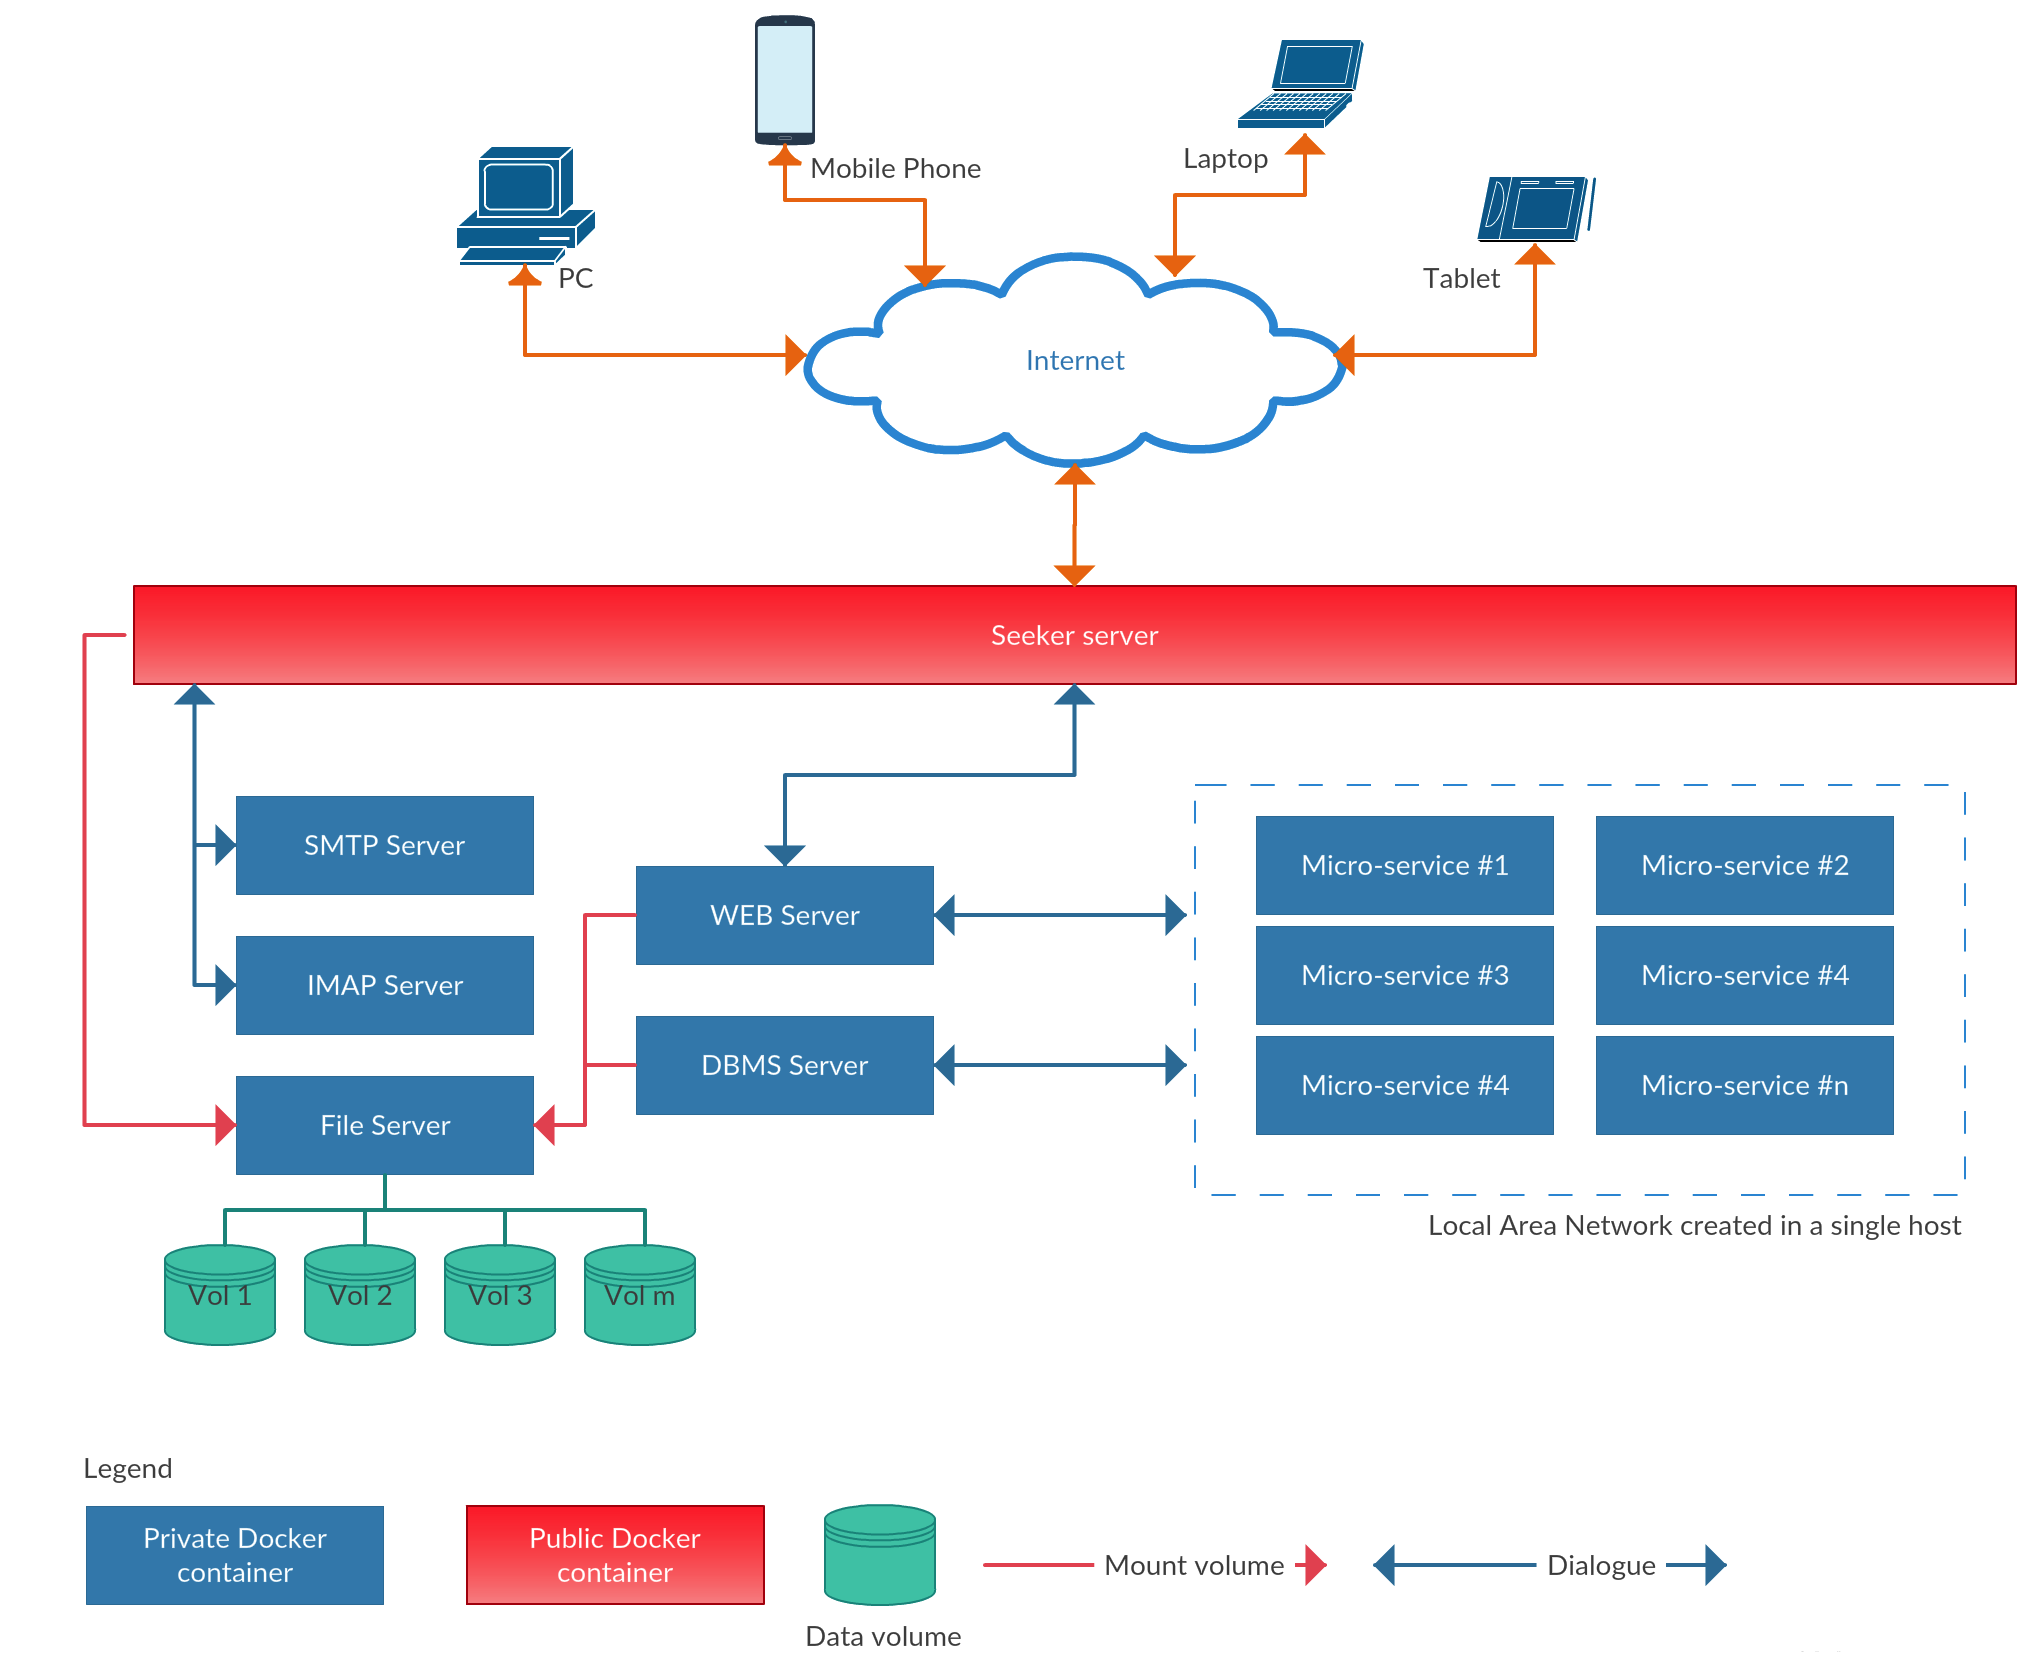
\includegraphics[width=1.2\textwidth, angle=90]{chapters/architecture/images/architecture.png}
	\caption[Proposed architecture]{Overview of a possible elastic and multi-tenant architecture that
		exploits the Docker containers.}
	\label{img:architecture-proposal-architecture}
\end{figure}

As we can see from the diagram, the architecture is composed by two different type of node:

\begin{itemize}
	\item{\keyword{private}: nodes that are only able to communicate with other nodes inside
		the same network;}
	\item{\keyword{public}: it is able to communicate with other nodes inside the same network
		and also accept incoming communication coming from Internet.}
\end{itemize}

A key component of our architecture is the \keyword{seeker server}. This is the key component that will
be able to manage all the elasticity requirements, we call it project ``ingress''. We will now describe
it.

\subsubsection{Ingress project}
\label{sec:architecture-proposal-architecture-ingress}
The main scope of the project is to provide a single and coherent access point, in which it is possible
to check all the incoming connection before they reach the \ac{vpn} network where the micro-services are
deployed.

Its main characteristics are:

\begin{itemize}
	\item{\keyword{security \& authentication}: it have to check, for each connection, all the necessary
		access requirements (loaded from a system database inside the File Server) before tenants are able
		to reach the desired resource;}
	\item{\keyword{monitoring}: it have to able to monitor the incoming traffic in order to correctly bill
		consumed resources to each tenant subscribed to the service;}
	\item{\keyword{dynamic routing}: it have to route each request to the most appropriate micro-service;}
	\item{\keyword{manage workload}: it have to manage the incoming workload in order to scale-in/scale-out
		micro-services only when necessary; it is also able to stop containers that have not incoming connection
		to manage\footnote{It is not convenient stop a container after each connection, but we have to build a
		technique like a ``watchdog''.};}
	\item{\keyword{static cache}: it is able to provide a static cache in order to reduce the latency time
		when clients access to static contents.}
\end{itemize}

This component will encapsulate a properly designed algorithm that on the basis of the actual workload
will be able to scale-in/out the necessary micro-services contained inside the private nodes (see Figure
\ref{img:architecture-proposal-architecture}). This algorithm will be based on the 
``monitor-analyse-plan-execute'' major cycle described in Section \ref{sec:elasticity-requirements-autonomy}.

Thanks to the increasing inclusion of the Docker \acs{api} inside the modern programming languages, will be
quite easy for this component to manage containers' life-cycle in order to replicate/close them when necessary.
Through managing containers' life-cycle we are able to scale our service and adapt it to current workloads

Another key point is in having a ``\keyword{filter battery}'' capable to ``\keyword{execute actions}'' on the
incoming requests if pre-determined criteria are satisfied. Figure 
\ref{img:architecture-proposal-architecture-ingress} shows a diagram that illustrate how each incoming request
will be manage before and after it reaches the service.

\begin{figure}
	\centering{}
	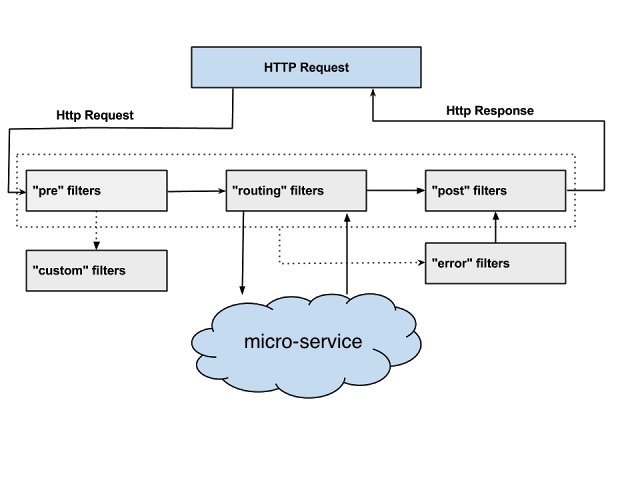
\includegraphics[width=0.8\textwidth]{chapters/architecture/images/ingress-design.png}
	\caption[Request management by ingress]{Algorithm that manage all the incoming requests to our
		services.}
	\label{img:architecture-proposal-architecture-ingress}
\end{figure}

The filter main characteristics are:

\begin{itemize}
	\item{\keyword{filter typlogy}: determine when the filter must be executed; possibility are:}
	\begin{itemize}
		\item{PRE: before the request reaches the micro-service, here we can make necessary security
			and authorization checks;}
		\item{ROUTING: decide to which micro-service route the incoming request, if the preceding
			checks performed successfully;}
		\item{POST: after the request reaches the micro-service, here we are to format the response
			before send it to the client;}
		\item{ERROR: in case a micro-service respond with an error code.}
	\end{itemize}
	\item{\keyword{order}: determine on which order filter on the same level will executed;}
	\item{\keyword{criteria}: the criteria that must be satisfied in order to apply the current filter;}
	\item{\keyword{action}: the associated action to the filter, executed only if the criteria results
		satisfied.}
\end{itemize}

As we argued this is the key component where the elasticity mechanisms are placed in order to guarantee
high level of performance and \ac{qos}.

\subsubsection{Micro-service network}
\label{sec:architecture-propoasal-architecture-network}
After having analysed the network costs (see Section \ref{sec:measurements-network-result}) we have
understood that it is necessary to locate containers with micro-services as much as possible inside 
the same physical host in order to reduce latency costs. Thus, we have decided to place the private
containers inside the same host linked together with the ``link'' capabilities provided by Docker
(see Section \ref{sec:background-deployments-docker-architecture}).

Creating a \ac{vpn}, as shown in Figure \ref{img:architecture-proposal-architecture}, with the
micro-services also increases the security performance because the exact network and micro-service
configuration will be hide to the outside world.To increase further the security performance we must
pay attention in creating connections only with the ``seeker'' node  or with nodes inside the same
\ac{vpn} (avoid connection over Internet as much as possible).

Finally, in order create good entry/exit points in each micro-service we want to adopt, as much as possible,
the \ac{amqp} protocol. This protocol avoid unnecessary synchronization between services allowing them
to serve multiple tenants concurrently.

\subsubsection{Multi-tenancy management}
\label{sec:architecture-propoasal-architecture-multiTenancy}
As we argued in Section \ref{sec:elasticity-multiTenancy} through good elasticity mechanisms developers
are able to provide multi-tenants applications or services to end-users and companies.

Given our decision to adopt the containerization as a base to support our architecture, and having 
understood the concepts illustrated in Section \ref{sec:architecture-soaRevisitation-microServices-requirements},
we focus our attention in building stateless micro-services, which they are easily shareable between
different tenants.

Micro-services have to contain the business logic of our application or service. Business logic is
the same between all tenants because there is not the presence of proprietary or sensible information\footnote{
	The business logic must process some meta-information, contained inside the incoming requests, that permit to
	distinguish different tenants.}. As a consequence there is the need of lower instances to support all tenants
(instead of having one replica of the service or application for each end-user).

The vertical separation, needed to maintain each tenant divided, must be managed in micro-services
which supervise the persistence layer (the ``File Server'' in Figure
\ref{img:architecture-proposal-architecture}). Exists mainly three possible techniques:

\begin{itemize}
	\item{\keyword{different database file}: each tenants access to a proprietary database file. This solution
		allow an easy schema customization and an high data separation that lead tenant to high level of security;}
	\item{\keyword{single database file multiple schemas}: each tenants access to same database file but access
		only to the associated schema; also in this scenario it is possible to easily customize the tenant's schema.
		In this scenario is more complicated restore data after a disaster because in the same file reside data of
		other tenants;}
	\item{\keyword{single database file single schema}: each tenants access to the same database file and schema.
		The tenants' data are separated by code placed inside the tables that compose the schema. This scenario is
		useful when we want lower costs and support an higher number of tenants by sacrificing some security aspects.
		In addiction, also in this case restore tenants' data after a disaster is more complicated because tenants'
		data are mixed together.}
\end{itemize}

As we just argued each one of the above techniques comes with its pro and cons. The architecture
proposed in Section \ref{sec:architecture-propoasal-architecture} can adopt each one of these
techniques. They represents different subscription type that differentiate the offered services.

Finally, to increase the overall performance will be possible to manage the Docker data-volumes
(see Section \ref{sec:background-deployments-docker-dataManagement}) through Flocker \cite{flockerHomepage}.
Flocker, shown in Figure \ref{img:architecture-proposal-architecture-multiTenancy-Flocker} gives to
ops-teams the tools they need to run containerized stateful services (like databases) in production
environments. Unlike a Docker data-volume which is tied to a single server, a Flocker data-volume,
called a dataset, is portable and can be used with any container in your cluster. Flocker manages Docker
containers and data-volumes together. When developers use Flocker to manage their stateful micro-service,
their volumes will follow the containers when they move between different hosts in the cluster.

\begin{figure}
	\centering{}
	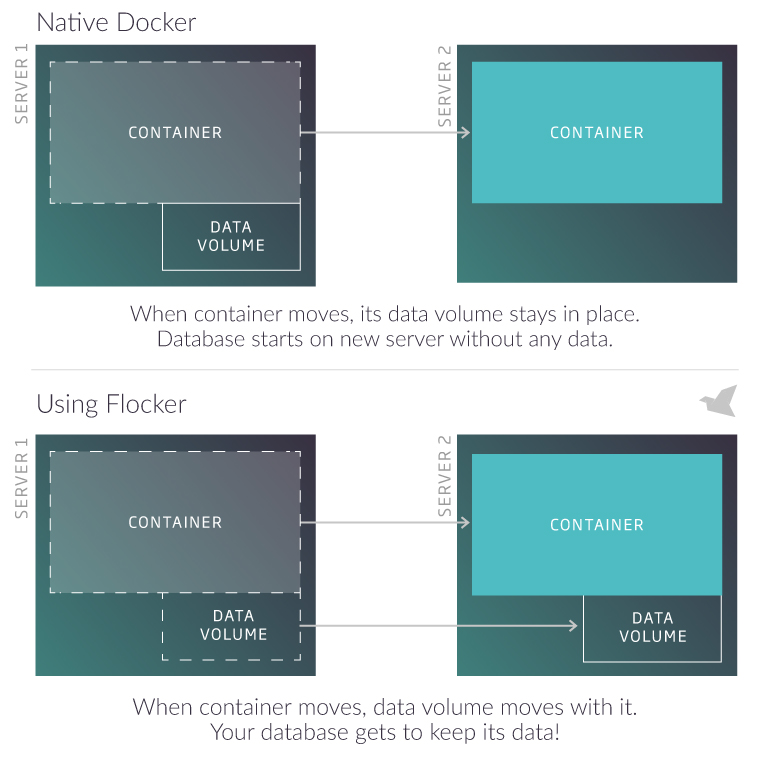
\includegraphics[width=0.6\textwidth]{chapters/architecture/images/flocker.png}
	\caption[Flocker capabilities]{When containers moves, data-volumes moves with it \cite{flockerHomepage}.}
	\label{img:architecture-proposal-architecture-multiTenancy-Flocker}
\end{figure}

\subsection{Related works}
\label{sec:architecture-related}
In literature we have also studied the work done by \citeauthor{baraldo2015reconciling} in
\cite{baraldo2015reconciling}. This is the work done during a preceding Master thesis that also wanted
to analyse the potentiality of the \ac{paas} layer.

The work done in the preceding thesis differs from our because they provide a framework that is able
to deploy an application or a service over differ \ac{iaas} cloud providers. Instead in our proposal
we have to base our service or application inside a \ac{paas} that offers Docker containers, like
Docker data centre (see Section \ref{sec:background-paas-platforms}).

\begin{figure}
	\centering{}
	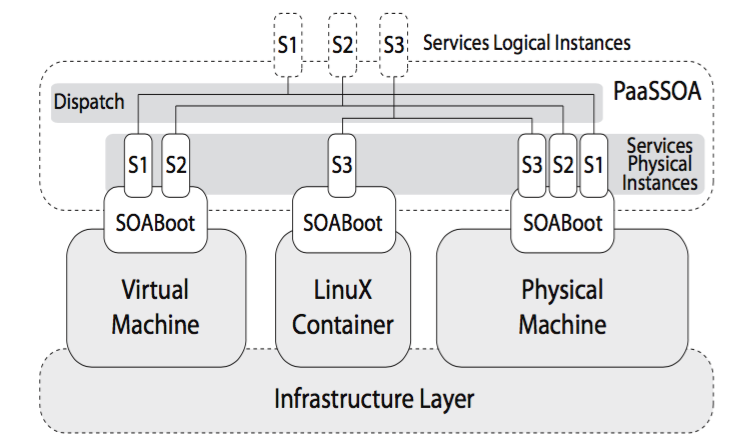
\includegraphics[width=0.6\textwidth]{chapters/architecture/images/passsoa.png}
	\caption[\acs{paas}\acs{soa} framework]{\acs{paas}\acs{soa} framework \cite{baraldo2015reconciling}}
	\label{img:architecture-proposal-related}
\end{figure}

In Figure \ref{img:architecture-proposal-related} we can see a high level overview of the \ac{paas}\ac{soa}
framework. \ac{soa}Boot agent are responsible for the deploying of a services inside a \ac{iaas} provider,
be it made by \ac{vm}, container or physical machines. It create a sort layer that is platform
independent.

%---------------------------------------------------------------------------------------------------
%		conclusion.tex
%
%	This is file contains an introduction about the SOA architectural desing.
%
%	Author: Andrea Meneghinello
% Version: 0.1
%	Table of changes:
%		21/03/2016 -> document definition
%---------------------------------------------------------------------------------------------------
\section{Conclusion}
\label{sec:architecture-conclusion}
In this thesis we tried to propose a possible a solution to simplify the necessary efforts to build
new software by developers.

As we argued in Section \ref{sec:background-problem} business companies do not want to manage the
necessary hardware to keep the application running according to the \ac{sla} requirements. Because
they will focus their efforts in the business and want to be supported by the software.

In the same section we also argued about the requests made by software-house which want to focus
their efforts in build and deploy software and not the environments to support it.

In this thesis we have learned that the \ac{paas} cloud model recently is becoming very interesting,
and in the nearly future the attention on it will increases again. This service model can answer to
both the set of requests made by companies and software-houses.

We have seen some basic capabilities offered by Docker containers and we have understood how they are
changing the \ac{paas} market. Many \ac{paas} providers in the market starting a migration to this
framework because it offers many useful functionalities and simplify the deployment model (see Section
\ref{sec:background-paas-platforms}). Even if we have seen, by the benchmark results in Chapter
\ref{cap:measurements}, that Docker container are less good in sharing the underlying hardware
assets, they are good to build elastic and multi-tenant service over the \ac{paas} cloud model
(see Chapter \ref{cap:architecture}).

With Docker we have available a powerful platform agnostic tool that permits to us to simply deploy
our applications and port them easily to different environments. With Docker, for software-houses
is easy to build home-made test environments when the software is under test and then deploy it in
a production environment. The only necessary thing is that both the environments have a running
Docker daemon.